\section{Introduction}\label{introduction}

\begin{quotation}
\textit{``There is no single development, in either technology or management technique, which by itself promises even one order-of-magnitude improvement within a decade in productivity, reliability, in simplicity.''} \citep[p.~1]{nosilverbullet}
\end{quotation}

Frederick P. Brooks, Jr. states this in his work \textit{No Silver Bullet} where he looks for a silver bullet to \textit{lay the werewolves of software complexity to rest} \citep[p.~1]{nosilverbullet}.

He breaks down software complexity and describes that reduction of software complexity is more feasible for some types of complexity than others.

This thesis explores the generation of user interfaces (UIs) for application programming interfaces (APIs) that fulfill certain criteria in the context of the World Wide Web. The main goal is to reduce the manual work in UI development by reducing complexity.

\subsection{Context}\label{context}
The context is UI development in web. These UIs are typically included in clients that run in browsers, on mobile devices or on desktop computers. They often exchange data with servers in the JSON data format \citep{jsonformat} through HTTP. The client is referred to as \textit{\gls{frontend}}, the server as \textit{\gls{backend}}. End users interact with those UIs to carry out tasks.

\subsection{Problem}\label{problem}
JSON is a popular format for data exchange between information systems in web development. Humans are able to infer the meaning of a piece of JSON data where machines are not. Specific knowledge about the JSON data is needed for a machine to understand the meaning of it. That specific knowledge is only valid for a certain API in a certain context. It is manually, often implicitly, encoded into the application containing the UI as shown in figure \ref{fig:hardcoded}. This knowledge is required to understand the data coming from such an API, it gives the data its semantics. These client applications are strongly coupled to specific APIs which hinders their re-use. Instead, client applications are written from scratch to work with slightly different APIs, often sharing the same or similar data models.

Current approaches fail to exploit the architecture of the World Wide Web and they completely ignore the possibilities offered by \gls{linkeddata}. These approaches we refer to as \textit{contemporary UI development}.

\begin{figure}[!htb]
  \center{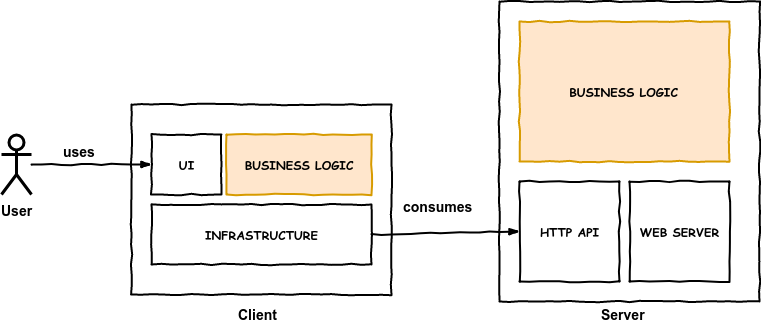
\includegraphics[width=450pt]
    {images/ui-dev-now.png}}
  \caption{The business logic is hard coded into the client.}
  \label{fig:hardcoded}
\end{figure}

\subsection{Scope and expected results}\label{sec:scope}
The main question that this thesis aims to answer is: \textit{Is it possible to reduce development costs in UI development by using \gls{linkeddata}?}

The scope and expected results of this thesis include following artifacts:

\begin{itemize}
\item a \gls{hypermedia} vocabulary or a HATEOAS specification
\item implementations of two HTTP APIs using that HATEOAS specification
\item a brief evaluation of design languages and their implementations
\item a proof of concept for the UI framework
\end{itemize}

The choice of the HATEOAS specification is driven by the implementation of the two HTTP APIs. The implementation of the HTTP APIs is driven by use cases that resemble real-world scenarios. A UI framework is implemented that is used to create a client that can consume HTTP APIs of both use cases. The framework uses a design language implementation internally to provide basic building blocks to the UI developer.

\subsection{Industrial partner}
The industrial partner of this thesis is M. Nieminen Consulting. M. Nieminen Consulting is interested in pushing open source efforts in \gls{linkeddata}-driven UI with complex user interaction. A future real-world use case is the generation of web-based back office applications for data and process management.
